\documentclass[11pt,oneside]{article}
\newcommand{\R}{\mathbb{R}}
\newcommand{\C}{\mathbb{C}}
\newcommand{\Z}{\mathbb{Z}}
\newcommand{\N}{\mathbb{N}}
\usepackage[french]{babel}
\usepackage[utf8]{inputenc}
\usepackage[T1]{fontenc}
\usepackage{lmodern}
\usepackage{array}
\usepackage{multicol}
\usepackage{titlesec}
\usepackage{graphicx}
\usepackage[margin=3cm]{geometry}
% \usepackage{fullpage}
% \usepackage{common}
\usepackage{amsmath,amsfonts,amssymb}
% \usepackage{overpic,boxedminipage}
\usepackage{hyperref}
\DeclareMathOperator*{\argmin}{arg\,min}
\DeclareMathOperator{\cotan}{cotan}
\DeclareMathOperator{\sinc}{sinc}
\DeclareMathOperator{\Tr}{Tr}
\DeclareMathOperator{\tr}{tr}
\DeclareMathOperator{\Gram}{Gram}
\DeclareMathOperator{\diag}{diag}
\newcommand{\lp}{\left(}
  \newcommand{\rp}{\right)}
\usepackage{blkarray}
\usepackage{multirow}
\usepackage{framed,fancybox}
\usepackage{tikz}
% \usepackage{algorithm2e}
% \usepackage{algorithmic}
\usepackage{float}
\usepackage{framed}
% \usepackage{ulem}
\usetikzlibrary{shapes,arrows}

\newcommand{\lela}{\left \langle}
  \newcommand{\rira}{\right \rangle}
\newcommand{\norm}[1]{\left\lVert#1\right\rVert}
\newcommand{\abs}[1]{\left|#1\right|}
\newtheorem{remarque}{Remarque}

\title{iXBlue}
\author{}
\date{}
\begin{document}
\maketitle
% \setcounter{secnumdepth}{1}
\setcounter{tocdepth}{1}
\tableofcontents

\section{Introduction}
% !TEX root = rapport.tex

%% Ecrit par David le 2 Mars 2015

Ce rapport résume les idées trouvées lors de la Semaine d'\'Etude Maths-Entreprises (SEME) qui a eu lieu du 12 au 16 janvier 2015 sur le problème proposé par iXBlue. Le problème initiale a été exposé de la manière suivante.\\
\textbf{\'Enoncé du problème proposé par iXBlue :} Un sous-marin sous l'eau ne peut pas connaitre sa position par GPS. Il doit donc déduire sa position à l'aide d'autres instruments de mesure, dont :
\begin{itemize}
	\item un accéléromètre qui lui donne son accélération au cours du temps $\vec{a}(t)$
	\item un appareil qui lui permet de mesurer la hauteur du fond marin (par rapport au niveau d'eau par exemple) au point où il se trouve.
\end{itemize}
On suppose de plus que le sous-marin possède dans sa mémoire interne une carte des fonds-marins (une fonction $H : \R^2 \to \R$ qui à un point de la surface $P = (x,y)$ associe la profondeur de l'eau en dessous de ce point $H(P)$). \\
Grâce à ces données, le sous-marin peut déduire sa position grâce à un algorithme dit \textit{de recalage} (cf Section \ref{sec:recalage}). On suppose maintenant que le sous-marin muni de son algorithme de recalage veut aller d'un point $A$ à un point $B$. Quelle est la meilleure trajectoire qui minimise l'incertitude en position au point final $B$ ? \\

Avant de commenter cette problématique, faisons quelques remarques. Le problème est deux-dimensionnelle, dans le sens où on peut toujours supposer que le sous-marin est à hauteur constante, et que les points $A$ et $B$ sont à cette hauteur. Ainsi, la trajectoire du sous-marin peut-être paramétrée par une fonction continue $\gamma : [0, T] \to \R^2$, où $\gamma(t)$ est la position du sous-marin au temps $t$. On a évidemment $\gamma(0) = A \in \R^2$, et $\gamma(T) = B \in \R^2$. Par ailleurs, afin de simplifier le problème, on supposera dans la suite que le sous-marin mesure sa vitesse $\vec{v}(t)$ et non son accélération (cela sera utile dans la suite pour avoir une croissance des erreurs en position en $O(t)$ et non en $O(t^2)$).\\

La problématique telle que précédemment formulée peut s'interpréter de multiples manières différentes. Il faut en particulier définir quelle est la notion d'incertitude. On supposera dans la suite que les appareils de mesure du sous-marin ne sont pas parfaits, et que l'incertitude vient uniquement de ces erreurs de mesure. Plus précisément, nous avons transformé le problème en un jeu à deux joueurs, dont un utilisateur externe et un sous-marin parfait muni d'un algorithme de recalage.\\

\textbf{Reformulation du problème en jeu à deux joueurs :}\\
\textbf{\'Etape 1} : L'utilisateur externe connait $A$ et $B$ et la carte des fonds marins, et il choisit un chemin $\gamma_0 : [0, T] \mapsto \R^2$ avec $\gamma_0(0) = A$ et $\gamma_0(T) = B$.\\
\textbf{\'Etape 2} : Le sous-marin connait $A$ et la carte des sous-marins. Il ne connait ni $\gamma_0$, ni $B$. Il va suivre \textbf{parfaitement} la trajectoire $\gamma_0$ et mesurer
\begin{itemize}
	\item sa vitesse (bruitée) ${\vec{\widetilde{v}}}(t) = \nabla \gamma(t) + \vec{e_v}(t)$, où $\vec{e_v}(t)$ est l'erreur en vitesse au temps $t$.
	\item la hauteur d'eau (bruitée) $\widetilde h(t) = h(\gamma(t)) + e_h(t)$, où $e_h(t)$ est l'erreur en hauteur d'eau au temps $t$.
\end{itemize}
Il estime ensuite avec son algorithme de recalage où il est à la fin (il estime la position de $B$).\\

Le but est alors pour l'utilisateur de trouver la meilleure trajectoire $\gamma_0$ telle que l'estimation soit la plus exacte possible. Notez que dans ce modèle, le sous-marin n'est pas soumis à la dérive, et suit exactement la trajectoire $\gamma_0$ imposée par l'utilisateur. Ce modèle peut paraitre simpliste, mais il permet déjà de mettre en avant les outils importants pour la résolution du problème. \\


Le point clé dans ce nouveau problème est que l'erreur vient uniquement des mesures (respectivement $\vec{e_v}(t)$ et $e_h(t)$). On supposera dans la suite que $\| \vec{e_v} \|_{L^\infty} \le \epsilon_v$ et $\| e_h \|_{L_\infty} = \epsilon_h$. Dans ce cas, pour une trajectoire donnée $\gamma_0 \in C^0([0,T], \R^2)$, il est naturel d'associer l'ensemble des trajectoires admissibles du sous-marin qui suit $\gamma_0$, à savoir
\[
	\mathcal{A}(\gamma_0) := \left\{ \gamma \in C^0([0,T],\R^2), \ \gamma(0) = A, \ \left\| \nabla \gamma (t) - \nabla \gamma_0(t) \right\|_{L^\infty} \le \epsilon_v, \ \left\| H(\gamma(t)) -  H(\gamma_0(t)) \right\| < \epsilon_h \right\}.
\]
Notez que la première condition traduit le fait que sous-marin connait sa point de départ $A$, que la seconde traduit le fait que son erreur en vitesse n'est pas plus grand que $\epsilon_v$, et que son erreur en hauteur d'eau n'est pas plus grand que $\epsilon_h$. Autrement dit, toute trajectoire de $\mathcal{A}(\gamma_0)$ est une trajectoire que le sous-marin peut penser prendre. On calcule ensuite l'ensemble des points finaux admissibles, à savoir
\[
	J(\gamma_0, T) := \left\{ \gamma(T), \quad \gamma \in \mathcal{A}(\gamma_0) \right\}.
\]
Avec ces notations, notre définition de l'incertitude est le volume de $J(\gamma_0, T)$, et le problème précédent peut s'écrire aussi
\[
	\textrm{Trouver} \quad \textrm{arginf} \left\{ | J(\gamma_0, T) |, \quad \gamma_0 \in C^0([0,T], \R^2), \ \gamma_0(0) = A, \ \gamma_0(T) = B \right\}.
\]
En pratique, la trajectoire $\gamma_0$ sera choisie avec des contraintes supplémentaires. On supposera par exemple que la vitesse du sous-marin est comprise entre $v_{\textrm min}$ et $v_{\textrm max}$, de sorte que $v_{\textrm min} \le | \nabla \gamma_0(t) | \le v_{\textrm max}$.  On supposera aussi que le temps $T$ est libre (autrement dit, la minimisation se fera aussi sur $T$). \\







Ce rapport est organisé comme suit. On commence par décrire un algorithme qui permet d'estimer l'incertitude (algorithme de recalage). Dans un second temps, nous donnons plusieurs solutions au problème sous forme discrète (qui correspond à des solutions ingénieries souhaitées par iXBlue), puis nous listons des pistes pour la résolution de problème sous forme continue, avec des approches déterministes et probabilistes.


















\section{Recalage}
\section{Optimisation de trajectoire}
\subsection{Deuxième algorithme de Dijkstra}
\subsubsection{Sélection de points}
\begin{figure}[hbtp]
\begin{center}
\begin{tikzpicture}[scale=0.5]
\draw[gray] (0,0) grid[xstep=0.125,ystep=0.125] (1,1);
\draw (0,0) grid (8,8);
\draw[->,>=latex] (-0.35,0.3) -- (0.2,0.3);
\draw node[left] at (-0.25,0.3) {$C$};
\end{tikzpicture}
\end{center}
\caption{Partitionnement de la carte de la bathymétrie}
\end{figure}

On propose un algorithme qui permet de sélectionner une partie des points de la carte qu'on considère intéressants. Réduire le nombre de noeuds du graphe est important car cela permet de réduire le coût de calcul de l'algorithme de Dijkstra. L'idée est que le recalage est a priori plus efficace lorsque la variation de la bathymétrie est importante autour du point où l'on effectue la mesure. Cet algorithme se décompose en quatre étapes
\begin{enumerate}
\item On effectue un partitionnement de la carte de bathymétrie.
\item On choisit un seuil $r\in (0,1)$.
\item Dans chaque sous partie $C$ , on sélectionne l'ensemble des points $P$ tels que $\|\nabla h(P)\|\geq \|\nabla h\|_{\mathit{L}^\infty(C)}(1-r)$.
\item On rajoute les points de départ et d'arrivée s'ils n'ont pas été sélection dans l'étape 3.
\end{enumerate} 
\begin{remarque}
Dans le cas où la bathymétrie est constante dans chacune des sous parties, l'algorithme sélectionne tous les points de la carte.
\end{remarque}
\begin{remarque}
Suivant le partitionnement de la carte et la valeur du seuil $r$, il n'est a priori pas garanti que le graphe puisse relier le point de départ et le point d'arrivée. Il faut rajouter des conditions sur la manière de partitionner et/ou le seuil qui seront à déterminer.
\end{remarque}

\subsubsection{Définition du coût}
Soient $P$ un noeud du graphe et $Q\in E_P$, on définit le coût associé à l'arète qui relie les deux points par
\begin{align*}
c(P,Q)=c(\{P,Q\}) \text{ pour tout }Q\in E_P.
\end{align*}
\subsection{Résultats}
Cette section présente les résultats des trois méthodes d'optimisation pour différents types de bathymétrie.

Le coût (le long de la trajectoire) de la trajectoire obtenue par l'algorithme glouton est plus grand que ceux obtenues avec les algorithmes de Dijkstra dans les différents cas considérés. L'approche globale de l'algorithme de Dijkstra est plus performante que la stratégie locale de l'algorithme glouton sur ce problème.

\subsubsection{Bathymétrie uniforme}
On considère la bathymétrie
\begin{align*}
h(x,y)=h_0.
\end{align*}
Cette carte de bathymétrie correspond au cas où le recalage ne nous donnerai pas d'information pour réduire la zone d'incertitude. Les résultats sont présentés dans la table \ref{tab_const}. 

\begin{table}
\begin{tabular}{cc}
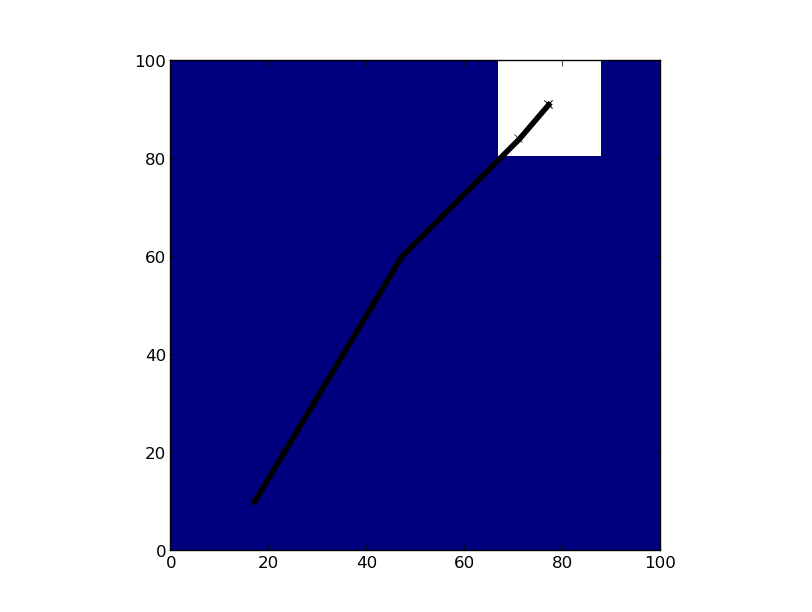
\includegraphics[scale=0.42]{../data/greedy_const/plot_A_10_17_B_91_77_iteration_010.png} &
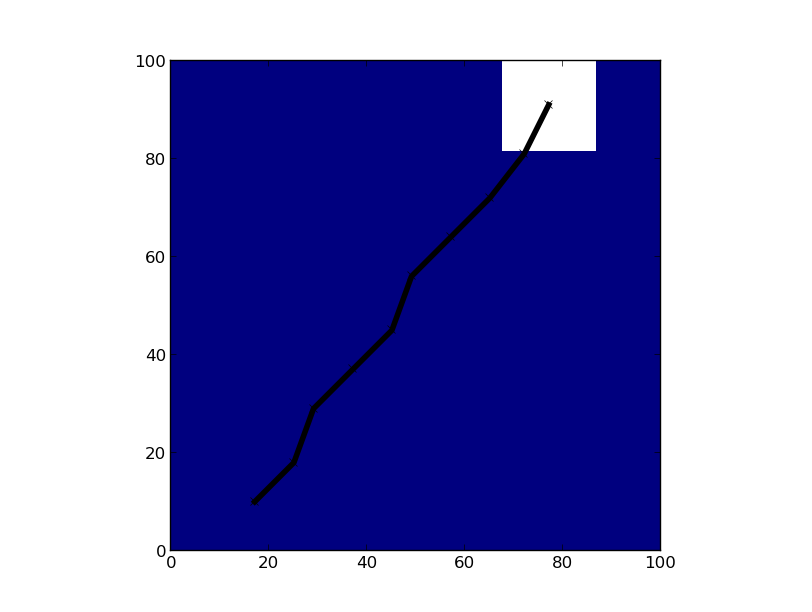
\includegraphics[scale=0.42]{../data/anneaux_const/plot_A_10_17_B_91_77_iteration_009.png} \\
Glouton, coût = 1749&Dijkstra 1, coût = 1329\\
&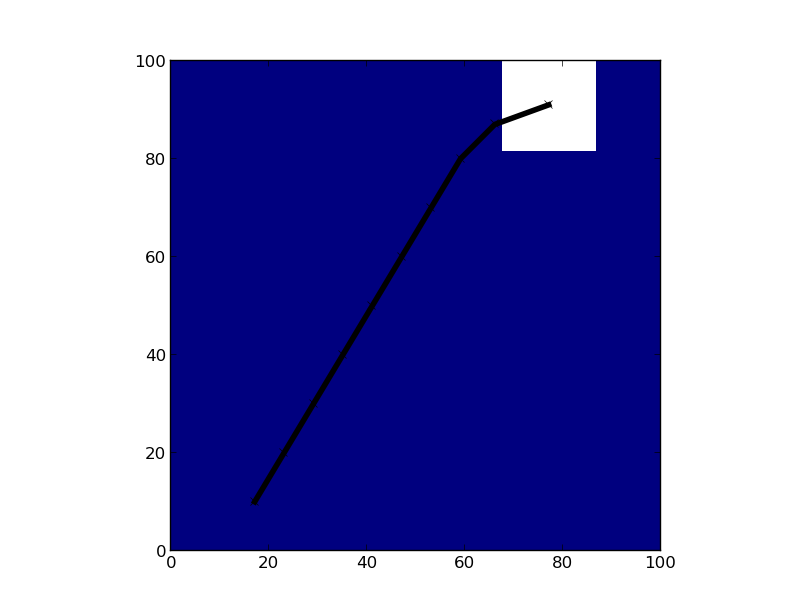
\includegraphics[scale=0.42]{../data/gradient_dijkstra_const/plot_A_10_17_B_91_77_iteration_009.png} \\
&Dijkstra 2, coût = 1329\\
\end{tabular}
\caption{Trajectoires, incertitudes à l'instant final et coût le long de la trajectoire}
\label{tab_const}
\end{table}
\subsubsection{Bathymétrie plane}
On considère la bathymétrie
\begin{align*}
h(x,y)=h_0 + \alpha y.
\end{align*}
 Les résultats sont présentés dans la table \ref{tab_plane}.
\begin{table}
\begin{tabular}{cc}
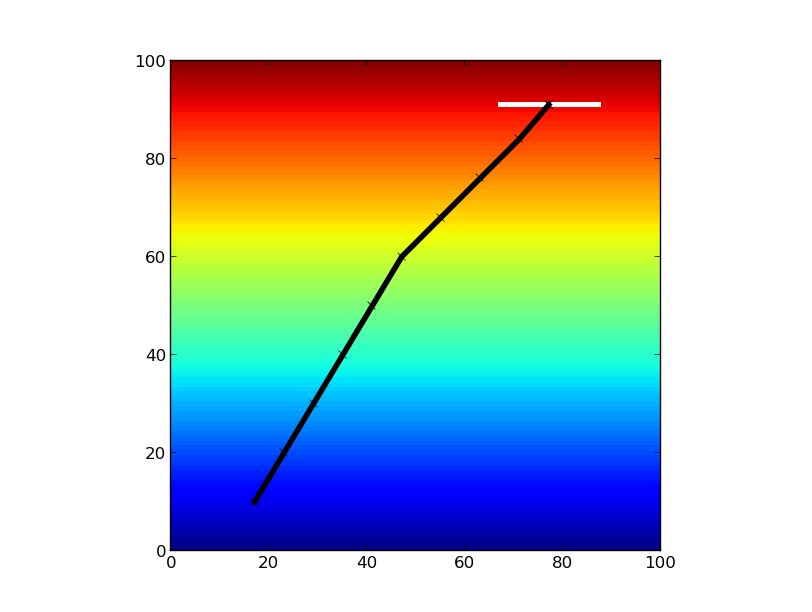
\includegraphics[scale=0.42]{../data/greedy_plane_2/plot_A_10_17_B_91_77_iteration_010.png} &
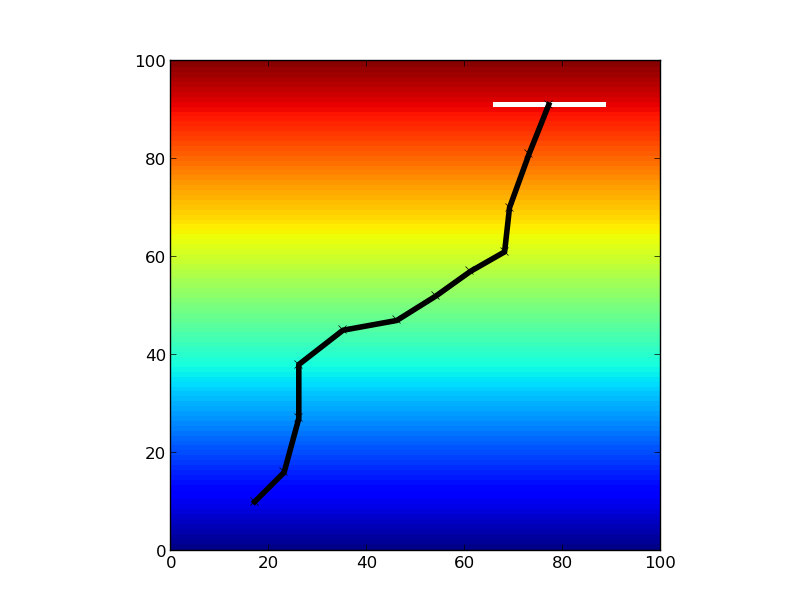
\includegraphics[scale=0.42]{../data/anneaux_plane_2/plot_A_10_17_B_91_77_iteration_011.png} \\
Glouton, coût = 120 &Dijkstra 1, coût = 69 \\
&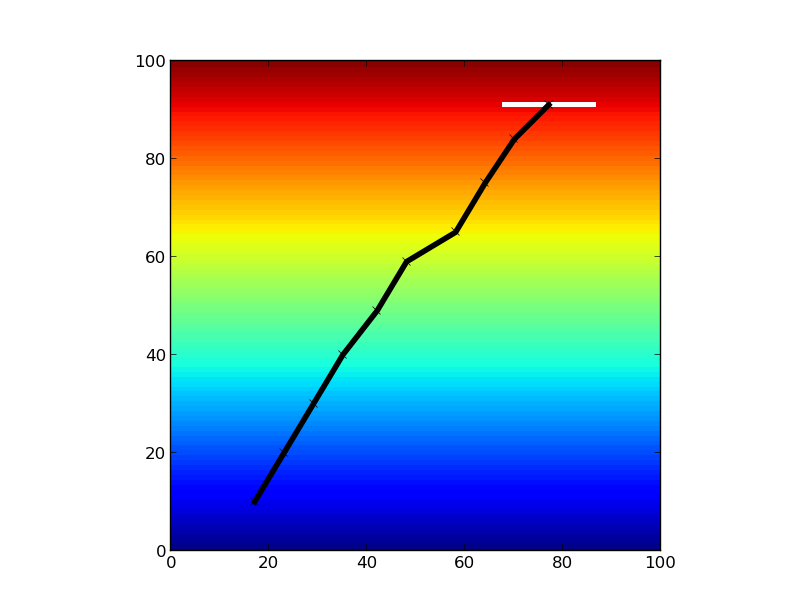
\includegraphics[scale=0.42]{../data/gradient_dijkstra_plane_2/plot_A_10_17_B_91_77_iteration_009.png} \\
&Dijkstra 2, coût = 99\\
\end{tabular}
\caption{Trajectoires, incertitudes à l'instant final, et coût le long de la trajectoire}
\label{tab_plane}
\end{table}
\subsubsection{Bathymétrie avec symétrie sphérique}
On considère la bathymétrie
\begin{align*}
h(x,y)=h_0-\alpha (x^2+y^2).
\end{align*}
 Les résultats sont présentés dans la table \ref{tab_cone}.
\begin{table}
\begin{tabular}{cc}
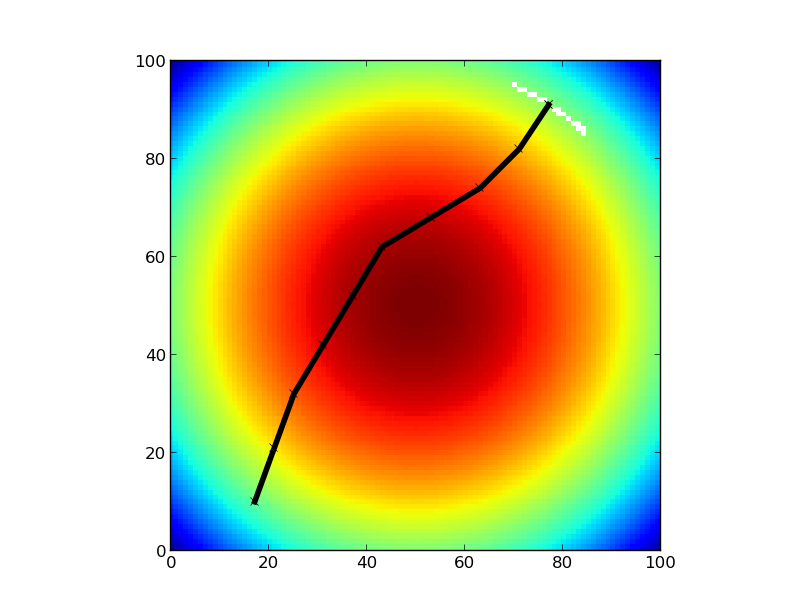
\includegraphics[scale=0.42]{../data/greedy_cone_2/plot_A_10_17_B_91_77_iteration_010.png} &
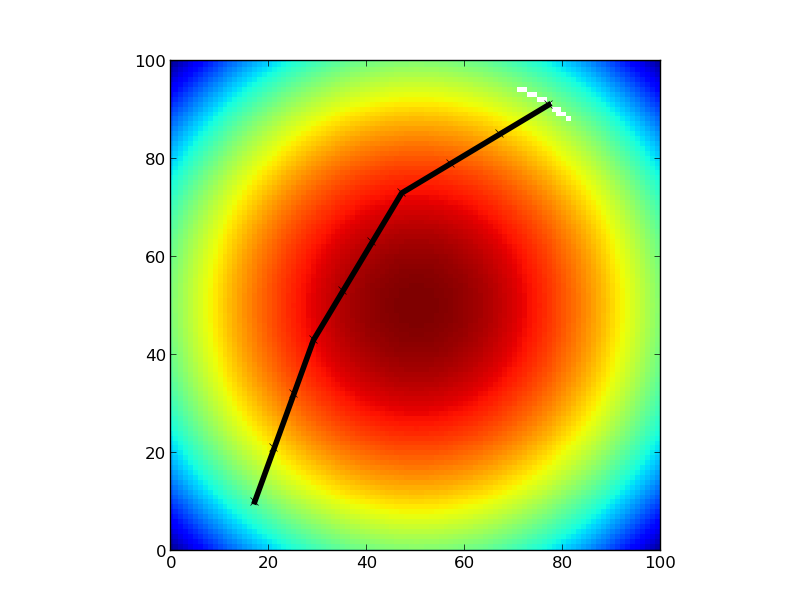
\includegraphics[scale=0.42]{../data/anneaux_cone_2/plot_A_10_17_B_91_77_iteration_009.png} \\
Glouton, coût = 178&Dijkstra 1, coût = 143\\
&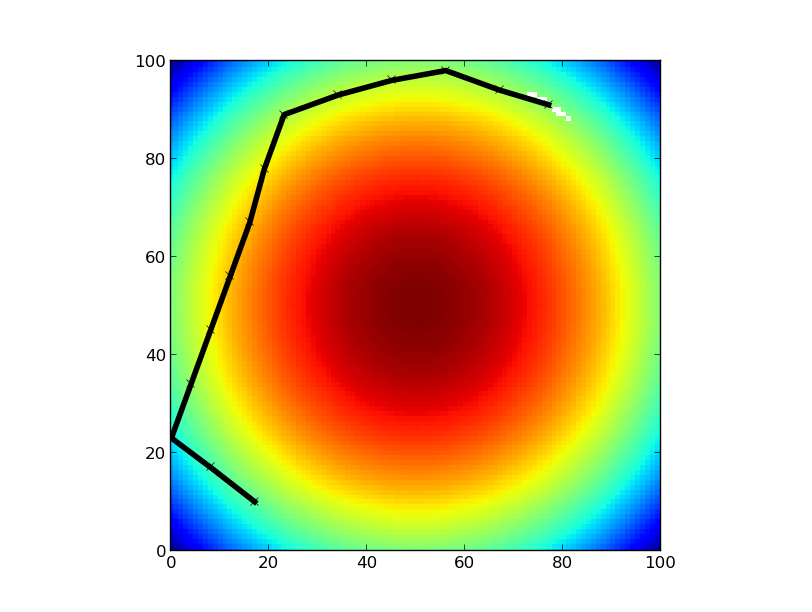
\includegraphics[scale=0.42]{../data/gradient_dijkstra_cone_2/plot_A_10_17_B_91_77_iteration_013.png} \\
&Dijkstra 2, coût = 129\\
\end{tabular}
\caption{Trajectoires, incertitudes à l'instant final et coût le long de la trajectoire}
\label{tab_cone}
\end{table}
\subsubsection{Bathymétrie de la morne rouge}
On considère la bathymétrie de la morne rouge. Les résultats sont présentés dans la table \ref{tab_morne}.
\begin{table}
\begin{tabular}{cc}
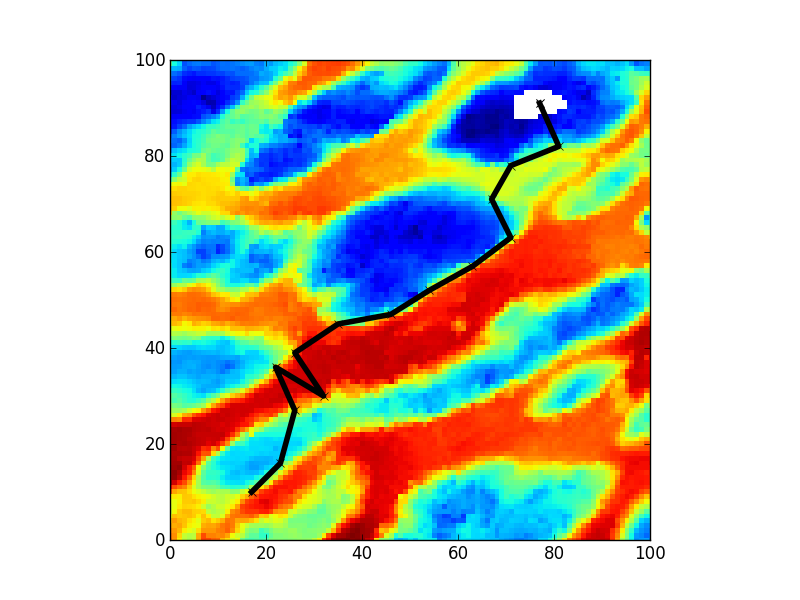
\includegraphics[scale=0.42]{../data/greedy/plot_A_10_17_B_91_77_iteration_015.png} &
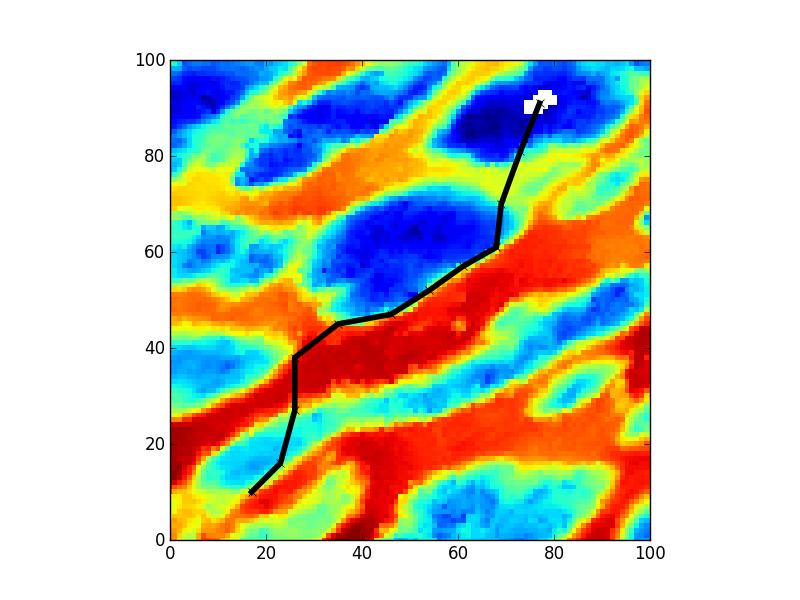
\includegraphics[scale=0.42]{../data/anneaux/plot_A_10_17_B_91_77_iteration_011.png} \\
Glouton, coût = 147&Dijkstra 1, coût = 69\\
&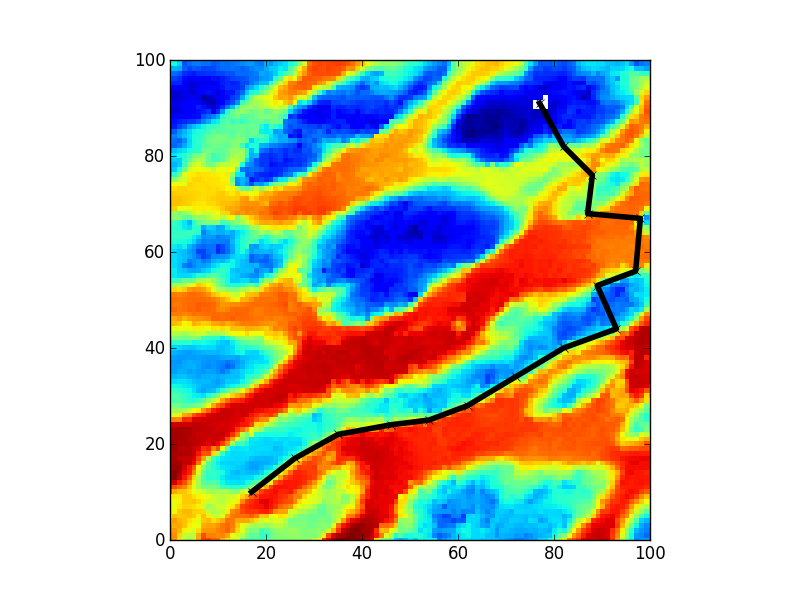
\includegraphics[scale=0.42]{../data/gradient_dijkstra/plot_A_10_17_B_91_77_iteration_015.png} \\
&Dijkstra 2, coût = 97\\
\end{tabular}
\caption{Trajectoires et incertitudes à l'instant final et coût le long de la trajectoire}
\label{tab_morne}
\end{table}


\section{Pistes continues}
\paragraph{Modèle jouet}
Les modèles précédents sont discrets par nature. Il est nécessaire de
se poser la question d'une modélisation continue (en espace et en
temps), soit qu'on espère que ces modèles sont les modèles limites des
précédents quand les échelles d'espace et de temps sont petites, soit
réciproquement pour obtenir de nouvelles idées d'algorithmes basés sur
une modélisation continue.

Dans cette partie, on suppose que la bathymétrie $h(x,y)$ est continue
et suffisamment régulière. L'inconnue est le chemin $\gamma : [0,1]
\to \R^{2}$, également supposé régulier.

Une première idée est de maximiser la pente parcourue, avec une
fonctionelle de type
  \begin{align*}
    c(\gamma) = -\int_{t=0}^{1} |\nabla h(\gamma(t))|^{2}  dt
  \end{align*}

  Ce problème est très mal posé: l'infimum n'est pas atteint, et les
  suites minimisantes se localisent sur les maximas de $\nabla h$, ce
  qui implique une perte de régularité de $\gamma$. Il
  est donc naturel de considérer une régularisation de ce problème
  pour éviter ce type de comportement pathologique, en pénalisant les
  $\gamma$ trop irréguliers :
\begin{align*}
  c(\gamma) =  \int_{t=0}^{1} a |\gamma'(t)|^{2} - b |\nabla
  h(\gamma(t))|^{2} dt
\end{align*}

Ce modèle nous semble être bien posé. Son étude mathématique et
numérique pourrait être intéressante, mais nous n'avons pas eu le
temps de la considérer. Cependant, il ne prend pas en compte
l'intuition (supportée par les simulations) que $\gamma$ doit alterner
les directions de $\nabla h$ pour localiser le sous-marin. Ce type
d'information nécessite une prise en compte de l'historique de
$\gamma$, et donc une fonction de coût non-locale, dont l'analyse est
plus compliquée.
% \begin{align*}
%   c(\gamma) =  \int_{t=0}^{1} a |\gamma'(t)|^{2} - b |\nabla
%   h(\gamma(t)) \cdot \gamma'(t)| dt
% \end{align*}

\paragraph{Un modèle un peu plus complexe}
Une autre possibilité est de modéliser l'évolution des incertitudes au
long de la trajectoire. Par exemple, en modélisant séparément les
incertitudes en $x$ et en $y$, on pourrait écrire
\begin{align*}
  c(\gamma) &= \sigma_{x}(1) + \sigma_{y}(1), \text{ où}\\
  \dot \sigma_{x} &= a - b \sigma_{x} (\partial_{x} h(\gamma(t)))^{2}\\
  \dot \sigma_{y} &= a - b \sigma_{y} (\partial_{y} h(\gamma(t)))^{2}.
\end{align*}

Ce modèle présente un amortissement exponentiel de $\sigma_{x}$ vers
un point d'équilibre
$\sigma_{x} \sim 1/(\partial_{x} h(\gamma(t)))^{2}$. Il est sous la
forme générale d'un contrôle optimal, et pourrait donc être traité par
ces méthodes (dont nous ne sommes pas spécialistes).

Un défaut de cette modélisation est que le modèle n'est pas isotrope
(il ne traite pas de la même façon les trajectoires dans des
directions différentes). Une généralisation possible pourrait être de
représenter l'incertitude par une matrice SDP $A$, dont les directions
et valeurs propres représenteraient une ellipse d'incertitude. Si on
pose $G = \nabla h \nabla h^{T}$, on peut considérer le modèle
\begin{align*}
  \dot A = a A - b \sqrt G A \sqrt G,
\end{align*}
analogue du précédent, mais traitant de la même façon toutes les
directions. On réduit ici les incertitudes dans la direction
$\nabla h$, et on ne les modifie pas dans la direction
$\nabla h^{\perp}$. Ce modèle est toutefois incohérent car $A$ ne
reste pas forcément SDP. Nous ne savons pas si il y a une ``bonne''
généralisation isotrope du modèle précédent.

\section{Pistes probabilistes}
\paragraph{Modélisation des incertitudes}
Dans toute l'étude précédente, on a pris pour postulat que les
incertitudes croissaient linéairement, sans trop se préoccuper des
mécanismes précis de cette croissance. D'où provient-elle, et comment
la modéliser ? Nous n'avons pas assez d'informations pour pouvoir
prétendre répondre à cette question, mais nous voyons plusieurs
sources d'erreur possibles : la précision de l'accéléromètre et des
gyroscopes, les erreurs d'intégration liées à la fréquence finie, et
les erreurs numériques en virgule flottante. Chacune de ces sources a
un comportement différent sur la dérive : une erreur initiale sur
l'accélération se traduit par une dérive en $t^{2}$, une erreur
initiale sur la vitesse se traduit par une dérive en $t$. Finalement,
dans le cas d'erreurs aléatoires se compensant, d'autres types
d'erreur, en $\sqrt t$, $t^{3/2}$ ou $t^{5/2}$ peuvent s'ajouter. La
prise en compte précise de ces croissances est importante pour bien
comprendre les incertitudes, le recalage, et les trajectoires
optimales.
\paragraph{Modélisation probabiliste}
Dans le cas d'erreurs aléatoires pouvant se compenser, la modélisation
précédente est trop pessimiste. On fait dans cette partie l'hypothèse
simplificatrice non-physique que les incertitudes proviennent d'une
mesure directe de vitesse entachée d'une erreur gaussienne
$N(0, \sigma_{v})$.

Supposons que le sous-marin suive la trajectoire $(x_{0}, x_{1} \dots,
x_{N})$, et notons $X_{n}$ la variable aléatoire représentant la
position estimée du sous-marin. Étant donnée la loi de $X_{n}$,
peut-on calculer la loi de $X_{n+1}$ ?

Sans recalage bathymétrique, on mettrait à jour la position
$X_{n + 1} = X_{n} + (x_{n+1} - x_{n}) + \varepsilon_{v}$, où
$\varepsilon_{v} \sim N(0, \sigma_{v})$ est une variable aléatoire
indépendante de $n$. Avec le recalage bathymétrique, on mesure
$h(X_{n+1}) = h(x_{n+1}) + \varepsilon_{h}$, avec une erreur
$\varepsilon_{h} \sim N(0, \sigma_{h})$. La loi de $X_{n+1}$ est donc 

  \begin{align*}
    X_{n+1} \sim L(X_{n} + v_{n} + \varepsilon_{v} \;\Big|\;
    h(X_{n} + v_{n} + \varepsilon_{v}) = h(x_{n+1}) + \varepsilon_{h})
  \end{align*}

  Si on note formellement $P(X=x)$ pour la densité de $X$ en $x$,
  \begin{align*}
    P(X_{n+1} = x) &= P(X_{n} + v_{n} + \varepsilon_{v} = x \;\Big|\;
    h(X_{n} + v_{n} + \varepsilon_{v}) = h(x_{n+1}) + 
                     \varepsilon_{h})\\
    &= \frac 1 N P(X_{n} + v_{n} + \varepsilon_{v} = x \cap
    h(X_{n} + v_{n} + \varepsilon_{v}) = h(x_{n+1}) + \varepsilon_{h})\\
    &= \frac 1 N P(X_{n} + v_{n} + \varepsilon_{v} = x) \; P(h(x) = h(x_{n+1}) + \varepsilon_{h}),
  \end{align*}
  où $N$ est choisi pour normaliser $X_{n+1}$.

  On peut donc calculer $P(h(x) = h(x_{n+1}) + \varepsilon_{h})$ (ce
  qui peut se faire facilement numériquement, et explicitement si on
  suppose $\varepsilon_{h}$ petit), puis calculer
  $P(X_{n} + v_{n} + \varepsilon_{v} = x)$ (par translation et
  convolution), multiplier et normaliser, ce qui nous donne la loi de
  $X_{n+1}$ en fonction de celle de $X_{n}$.

  Cette approche, uniquement intéressante si les incertitudes sont
  bien modélisées par des déviations aléatoires indépendantes, est
  moins pessimistes que l'approche par boites, et permet des
  intervalles de confiance plus resserrés. Enfin, ce type d'approche
  est peut-être lié à des approches par filtre de Kalman, mais ces
  liens dépassent nos compétences et le cadre de notre étude.

\section{Conclusion}
\section{Bibliographie}
\end{document}
